\documentclass[17pt]{beamer}
\usetheme{metropolis}
\usepackage[utf8]{inputenc}
\usepackage{graphicx}
\usepackage[german]{babel}
\usepackage{wrapfig}
\usepackage{blindtext}


%Information to be included in the title page:
\title{STM32 Webserver}
\author{Harald Korinek - Samuel Teufel - Valentin Veluppillai}
\date{}

\begin{document}

\frame{\titlepage}
%--- Next Frame ---%

\begin{frame}[t]{Ziel}
  Semester:\\
  Realisierung eines Webservers auf einem STM32 uC.


  Diplomprojekt:\\
  Entwicklung einer Plattform für Automatisierung und Webanbindung von Messgeräten
\end{frame}
%--- Next Frame ---%

\begin{frame}[t]{IDE}
  \vspace{25pt}
  \begin{itemize}
    \item Atollic TrueStudio
    \item CubeMX
    \item CubeIDE
  \end{itemize}
\end{frame}
%--- Next Frame ---%

\begin{frame}[t]{Systemübersicht}
  \centering
  \begin{figure}
    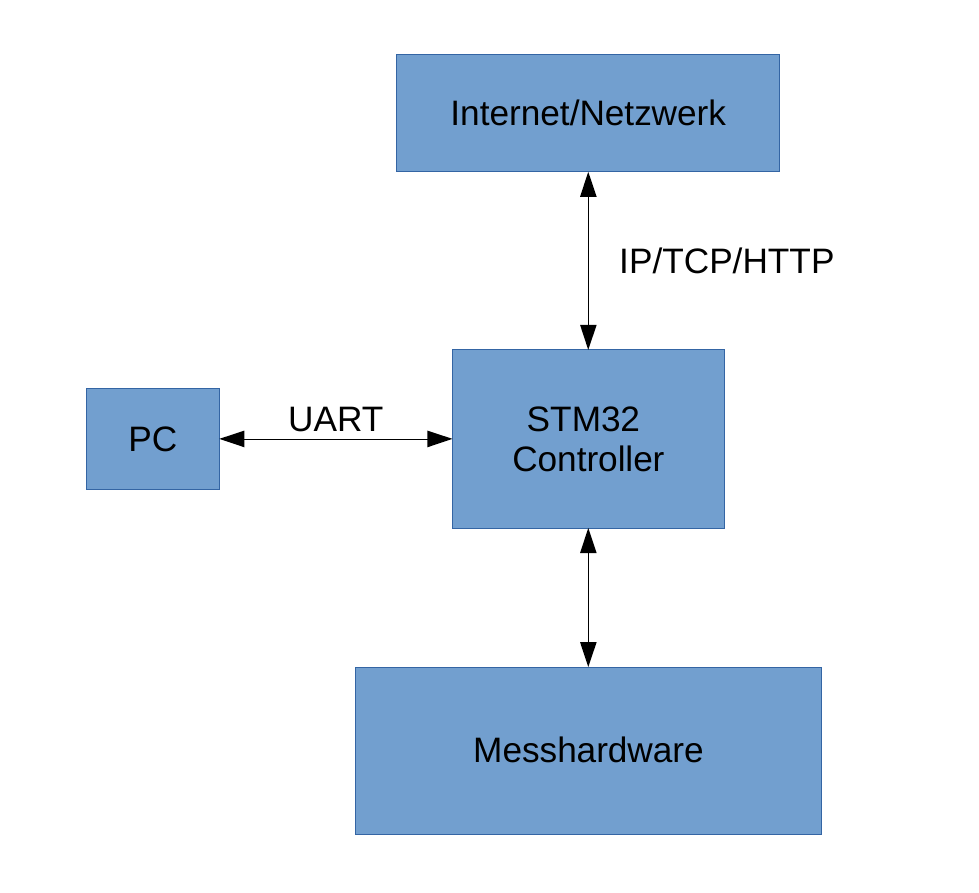
\includegraphics[height=0.8\textheight]{images/block_schematic}
  \end{figure}
\end{frame}
%--- Next Frame ---%

\begin{frame}[t]{lwIP}
  \vspace{2cm}
  \begin{itemize}
    \item lightweight TCP/IP Stack
    \item ermöglicht einfache Internetanbindung
  \end{itemize}
\end{frame}
%--- Next Frame ---%

\begin{frame}[t]{RTOS}
  \vspace{2cm}
  \begin{itemize}
    \item mbedOS
    \item FreeRTOS
  \end{itemize}
\end{frame}
%--- Next Frame ---%

\begin{frame}[t]{Realisierung}
  \vspace{10pt}
  \begin{itemize}
    \item Kennenlernen der STM32-Familie
    \item FreeRTOS
    \item STM32-Hardware
    \item lwIP
    \item Integration
  \end{itemize}
\end{frame}
%--- Next Frame ---%

\begin{frame}[t]{UART und Webserver}
    \centering
    \vspace{0.1\textheight}
    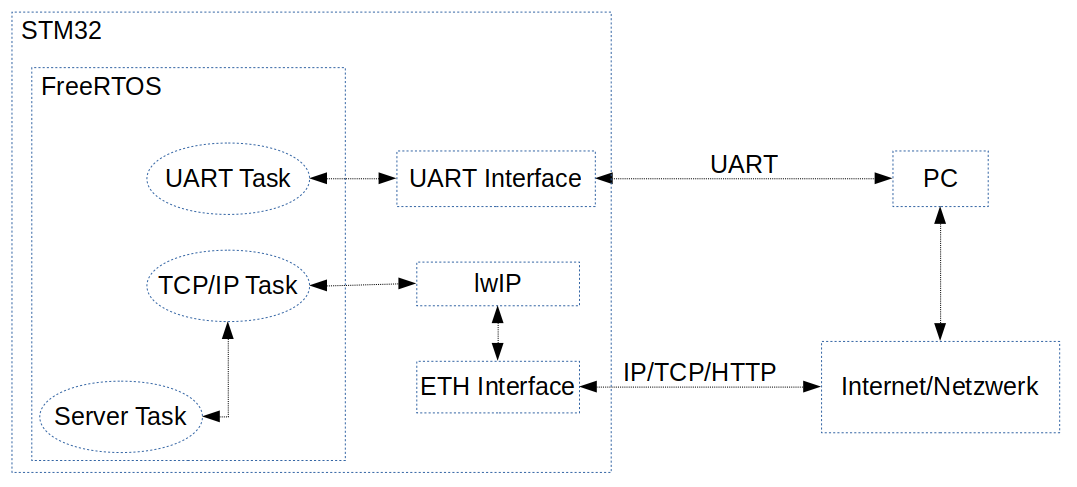
\includegraphics[width=\textwidth]{images/webserver_block}
\end{frame}
%--- Next Frame ---%

\begin{frame}[t]{Rotary Encoder und PWM}
  \centering
  \vspace{0.1\textheight}
  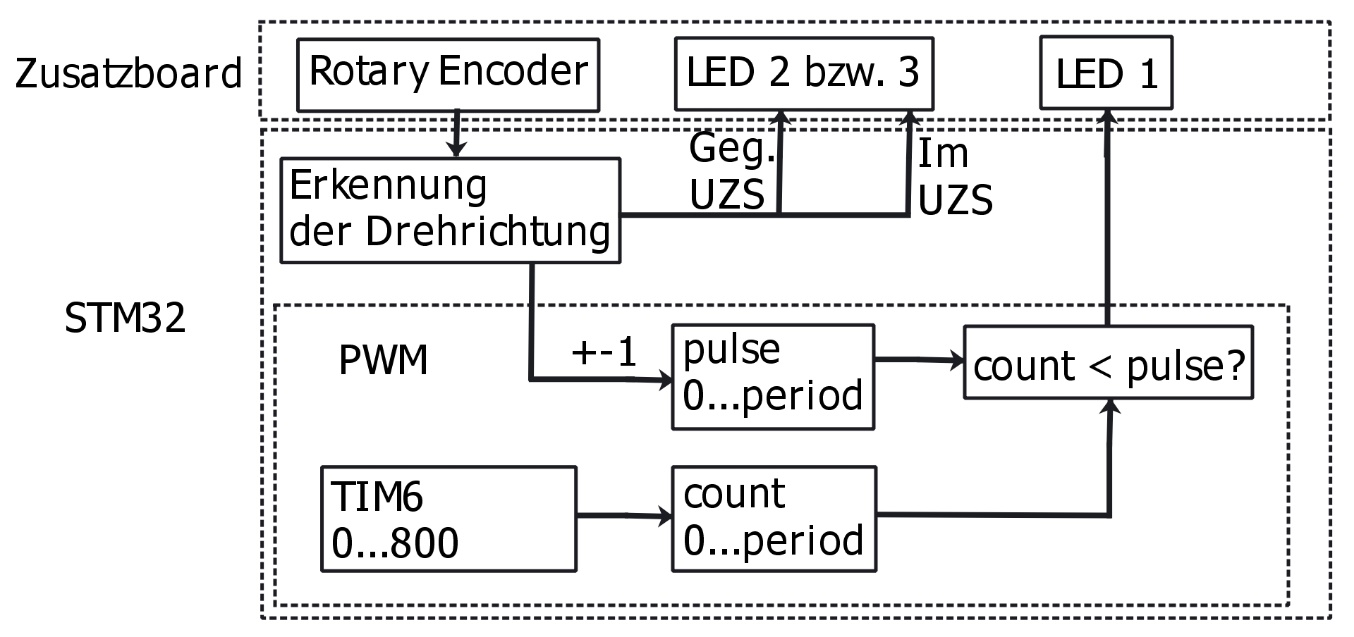
\includegraphics[width=\textwidth]{images/rotary_block}
\end{frame}
%--- Next Frame ---%

\begin{frame}[t]{Extension Board}
  \begin{tabular}{cl}
      \begin{tabular}{c}
           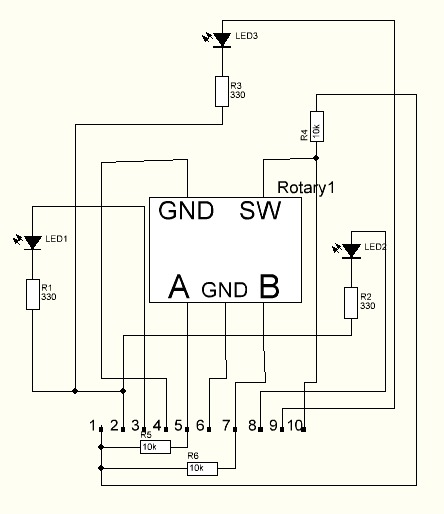
\includegraphics[height=0.8\textheight]{images/schem}
      \end{tabular}
      \begin{tabular}{l}
          \parbox{0.5\linewidth}{
            \begin{tiny}
              \begin{enumerate}
                  \item 5V Pullup
                  \item LED GND
                  \item LED1 VCC
                  \item Rotary Switch GND
                  \item A-Ausgang
                  \item A/B Referenz
                  \item B-Ausgang
                  \item LED2 VCC
                  \item LED3 VCC
                  \item Rotary Switch
              \end{enumerate}
            \end{tiny}
            }
      \end{tabular}
  \end{tabular}
\end{frame}
\end{document}
